\section{Results}

The controllers have been simulated in MATLAB Simulink in order to generate results presented in this section. 

The model parameters can be seen in \autoref{ParametersQuadcopter}. All of them have been obtained through test but the moments of inertia, which were calculated with following an analytical procedure.

\begin{table}[H]
    \centering
    \begin{tabular}{c|c|c}
        %------------------------------------------------------------------------------------------
        \textbf{Symbol} &\textbf{Value} &\textbf{Units}\\
        \hline %-----------------------------------------------------------------------------------
        $m$ & 0.996       &$kg$\\
        \hline %-----------------------------------------------------------------------------------
        $L$  &   0.225       & $m$\\
        \hline %-----------------------------------------------------------------------------------
        $J_x$  & 0.01073       & $kg \  m^2$\\
        \hline %-----------------------------------------------------------------------------------
        $J_y$  & 0.01073       & $kg \  m^2$\\
        \hline %-----------------------------------------------------------------------------------
        $J_z$  & 0.02135       & $kg \  m^2$\\
        \hline %-----------------------------------------------------------------------------------
        $k_{th}$  & 1.32922\ $10^{-5}$       & $N \  s^2 \  rad^{-2}$\\
        \hline %-----------------------------------------------------------------------------------
        $k_{d}$  & 9.39741\ $10^{-7}$       & $N \  m \  s^2 \  rad^{-2}$\\
        \hline %-----------------------------------------------------------------------------------
        $\overline{\omega}_i$& 429      & $rad \ s^{-1}$\\
        
    \end{tabular}
    \caption{Parameters used though the analysis and design.}

    \label{ParametersQuadcopter}
\end{table}
The attitude controller is defined chosen feedback and integral poles and the observer poles. These are chosen to be $[-6 -6.2 -6.4 -6.6 -6.8 -7 -7.2 -7.4 -7.6]$ and $[-20 -25 30]$ respectively.

The translation velocity controllers of the x and y translational are $C_{\dot{x}}(s)= -0.1$, $C_{\dot{y}}(s)= 0.1$ and the position ones are $C_x(s)= 0.5$, $C_y(s)= 0.5$. The inner loop proportional controller of the z translational cascade controller is
$C_{\dot{z}}(s)=\frac{-201s+0.8}{s}$ and the outer loop is $C_z=0.9$

This controllers have been discretized using th Tustin method with a sampling period of 30 ms. 

Regarding the network, the mean delay selected is 30 ms and the package loss probability has been set to 0 due to the low sending frequency used in the system.
The simulation results obtained with these parameters and controllers are shown in \autoref{PositionControl}.
\begin{figure}[H]
	\centering
	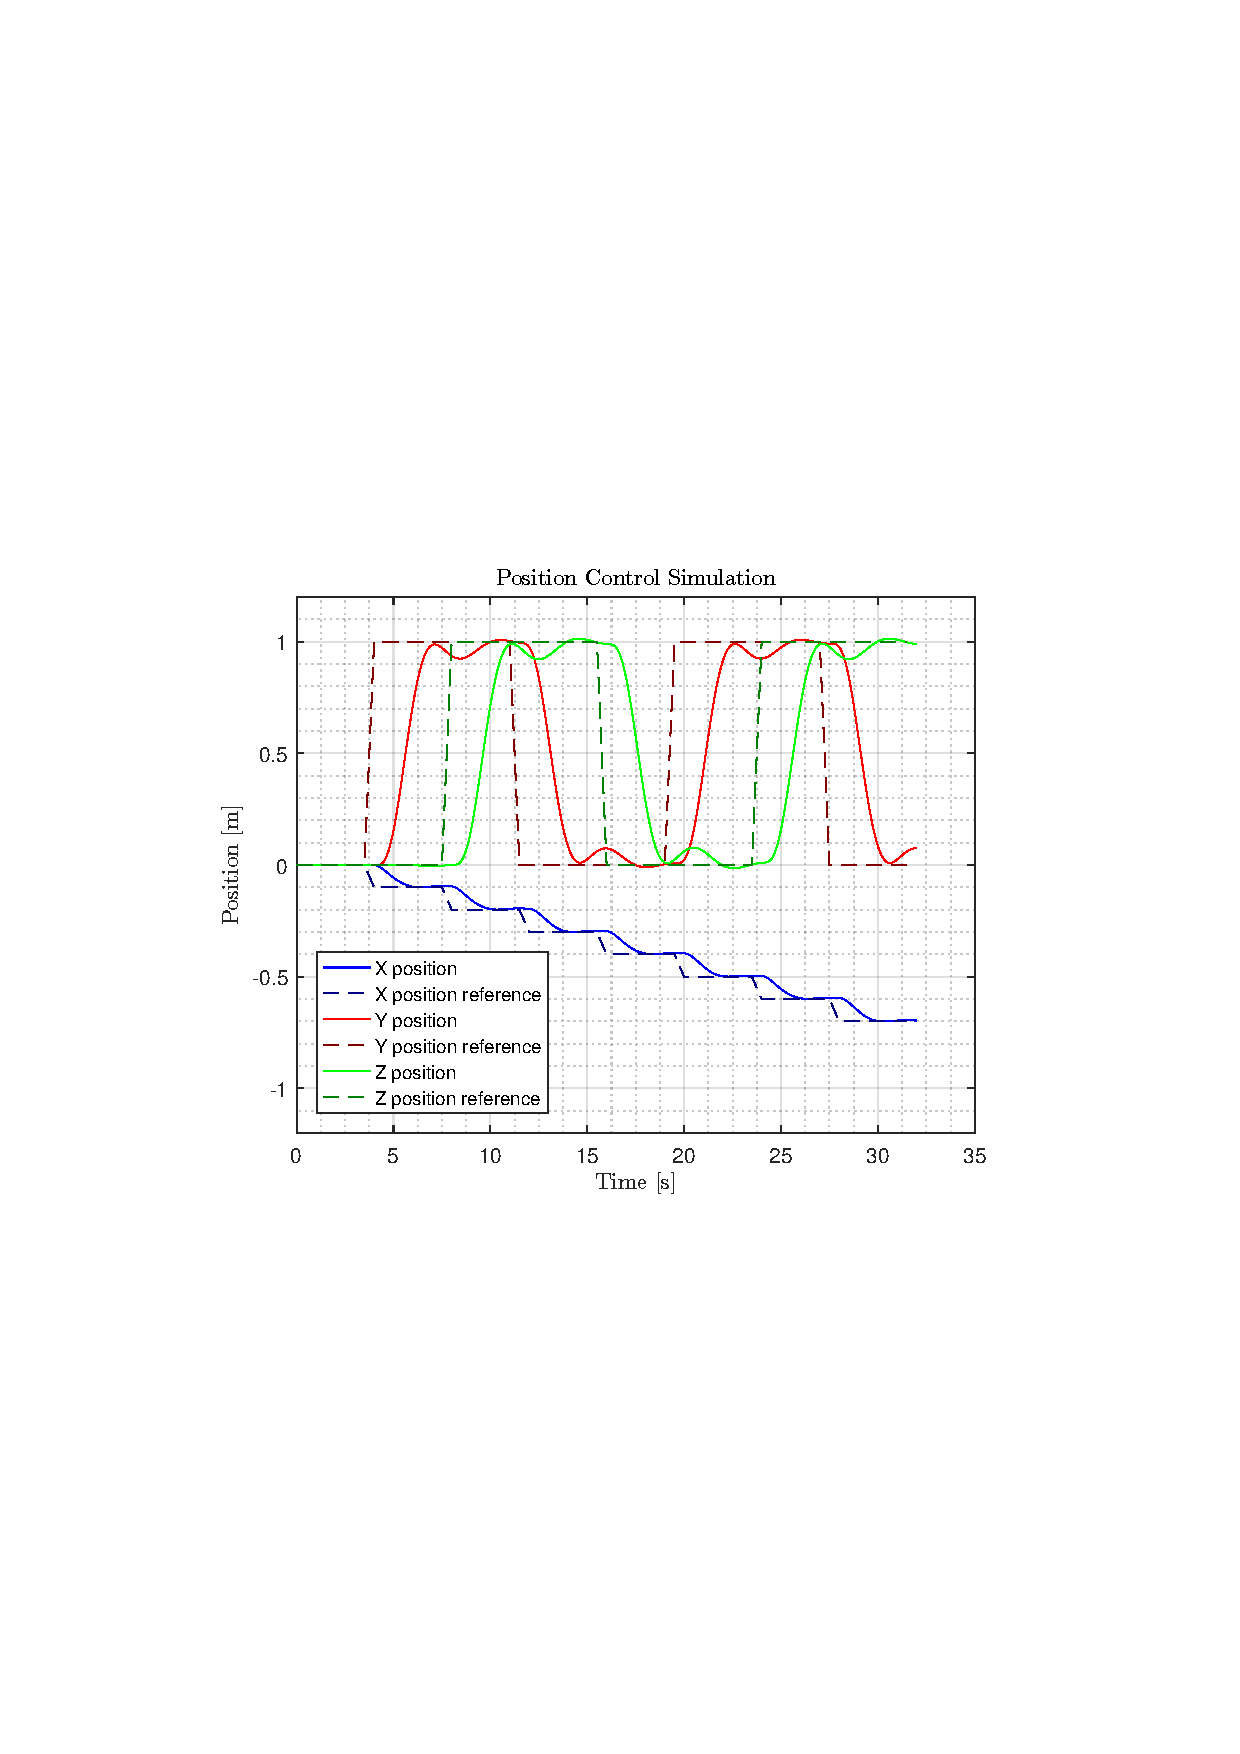
\includegraphics[scale=0.5]{figures/PositionControl}
	\caption{Position control results in the three inertial axes directions. The references given to the control system are shown with dashed lines.}
	\label{PositionControl}
\end{figure}

The inner attitude controller results are also included in and shown in \autoref{AttitudeControl} so the performance of the attitude control can be evaluated. 
\begin{figure}[H]
	\centering
	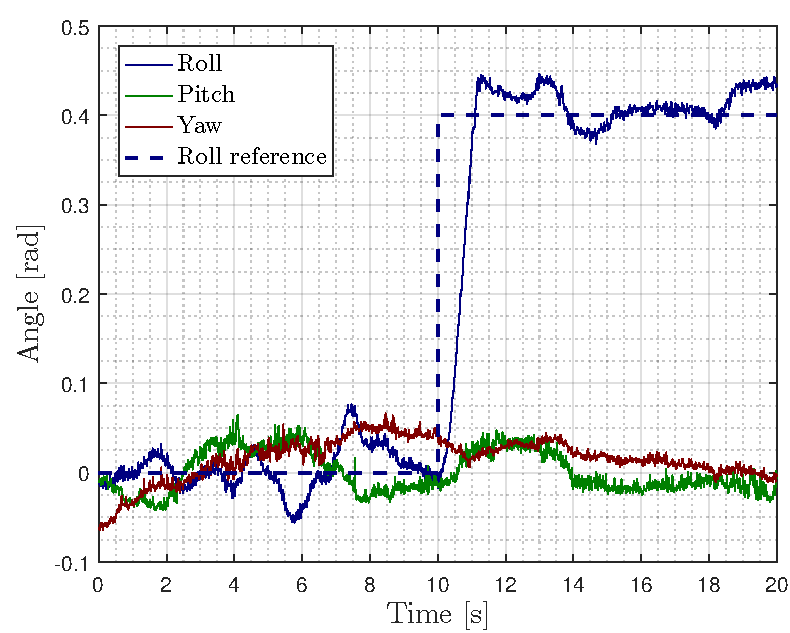
\includegraphics[scale=0.5]{figures/AttitudeControl}
	\caption{Attitude control results in the three angles. The references given to the attitude control system are shown with dashed lines.}
	\label{AttitudeControl}
\end{figure}


